\documentclass[11pt]{amsart}
\usepackage{amsmath,amssymb,amsthm,mathtools}
\usepackage[margin=1in]{geometry}
\usepackage{booktabs}
\usepackage{array}
\usepackage{enumitem}
\usepackage{tikz}
\usetikzlibrary{positioning,arrows.meta}
\usepackage[colorlinks=true,linkcolor=blue,citecolor=blue]{hyperref}

\newcommand{\Gs}{G^{*}}
\newcommand{\GG}{G_{\!\scriptscriptstyle\mathrm{G}}}
\newcommand{\GK}{G_{K}}
\newcommand{\Z}{\mathbb{Z}}
\newcommand{\Q}{\mathbb{Q}}
\newcommand{\R}{\mathbb{R}}
\newcommand{\C}{\mathbb{C}}
\newcommand{\Aut}{\mathrm{Aut}}

\title{The $\Gs$ opus: a four-paper overview\\
\large Reader's guide, dependency map, and submission strategy}
\author{}
\date{2026-05-19}

\begin{document}
\maketitle

\section*{Summary in one paragraph}

The lemniscatic constant $\Gs = \Gamma(1/4)/\Gamma(3/4) \approx 2.95867$
and its Gaussian-AGM partner $\GG = 1/\mathrm{AGM}(1,\sqrt 2) \approx 0.83463$
are two normalisations of the same transcendental quantity at the CM point
$\tau = i$. This opus organises every algebraic and analytic identity in
their neighbourhood as the projection at four arithmetic levels of a
single Kronecker character $\chi_{-4}$ on $(\Z/4\Z)^{\times}$, extends the
construction to the full atlas of class-number-one imaginary quadratic
fields ($d \in \{1, 2, 3, 7, 11, 19, 43, 67, 163\}$), and proves a clean
$\eta$-tower theorem $|\eta(\tau_K)|^{2 w_K} = \GK^{w_K}/(2\pi|d_K|)^{w_K/2}$
that uniformly recovers the lemniscatic case and the Heegner near-integer
phenomenon $e^{\pi\sqrt{163}} \approx 640320^{3} + 744$ as instances of
the same arithmetic structure. The opus consists of four papers, total
$44$ pages of new mathematics, with the master quadratic uniqueness
theorem and the value-algebra polynomial-ring statement as the principal
structural results.

\section{The four papers}

\begin{center}
\renewcommand{\arraystretch}{1.3}
\begin{tabular}{>{\bfseries}l l c l}
\toprule
Paper & Title (abbreviated) & Pages & Target venue \\
\midrule
A & \emph{The Kronecker character $\chi_{-4}$ as the joint source of the lemniscatic identity algebra} & 29 & Crelle / Compositio / Math.\ Ann.\ / JLMS \\
B & \emph{The master quadratic $P_{\Gs}$ as a math--physics bridge} & 5 & Foundations of Physics \\
C & \emph{The class-number-one atlas: nine CM constants and their $\chi$-unifications} & 6 & J.\ Number Theory / Acta Arithm.\ \\
D & \emph{The $\eta$-tower across the class-number-one atlas} & 4 & J.\ Number Theory / Math.\ Comp.\ \\
\bottomrule
\end{tabular}
\end{center}

All four are LaTeX-compiled, internally cross-referenced, and verified to
50--80 digit numerical precision. Paper A contains the structural spine
(50+ identities, the $\chi_{-4}$-unification theorem, the $\eta$-half-tower,
quasi-modular value algebra, equianharmonic dichotomy, the master
quadratic with its $(2, 3)$ uniqueness theorem). Papers B--D are short
companions that extend particular threads.

\section{The mathematical spine: $\chi_{-4}$, the master quadratic, the atlas}

The opus has two unifying structural results.

\paragraph{The four-level unification (Paper A \S 16).} The Kronecker
character $\chi_{-4}: (\Z/4\Z)^{\times} \to \{\pm 1\}$ generates the
entire $\Gs/\GG$ identity ring through four functorial projections:
\begin{enumerate}[label=\textup{(L\arabic*)}, leftmargin=*, itemsep=2pt]
\item \emph{Lattice}: $|\Z[i]^{\times}| = 4 = $ squared coefficient in the master quadratic;
\item \emph{Chowla--Selberg}: $\prod_{a} \Gamma(a/4)^{\chi_{-4}(a)} = \Gs$;
\item \emph{Hecke}: $a_p \neq 0$ iff $\chi_{-4}(p) = +1$ in $L(E_{\mathrm{lemn}}, s)$;
\item \emph{Dirichlet}: $L(\chi_{-4}, 1) = \pi/4$ (Leibniz).
\end{enumerate}
The mutual consistency of (L2)--(L3) is Deligne's period conjecture
restricted to the CM case (proved by Blasius, Anderson, Shimura).

\paragraph{The atlas extension (Paper C).} Each of the nine
class-number-one imaginary quadratic fields $K = \Q(\sqrt{-d})$ admits a
canonical Chowla--Selberg constant
$\GK := \prod_{a} \Gamma(a/|d_K|)^{\chi_{d_K}(a)\,w_K/4}$
parameterised by the discriminant and unit order. The lemniscatic
$\Gs = G_{\Q(i)}$ and the equianharmonic $R_{3}^{3/2} = G_{\Q(\rho)}$
are the only two with $w_K > 2$ and hence the only two supporting a
dual-constant dichotomy.

\paragraph{The master quadratic uniqueness (Paper A \S 16.5, Theorem).}
Among polynomials of the form $x^{2} - 16\,{\Gs}^{a}\,x + 16\,{\Gs}^{b}$
($a < b$ positive integers), the pair $(a, b) = (2, 3)$ is the unique
minimal-$a$ choice whose roots are not scalar multiples of any single
period ${\Gs}^{k}$. (Restriction: leading-period polynomials. The general
case where coefficients range over $\mathrm{Sym}^{a}H^{1}$ remains as
Conjecture 16.5.2.)

\section{Reading order by audience}

\begin{center}
\renewcommand{\arraystretch}{1.25}
\begin{tabular}{>{\bfseries}l l}
\toprule
Audience & Recommended reading path \\
\midrule
CM theorist / number theorist & Paper A \S 1--\S 16 $\to$ Paper C $\to$ Paper D $\to$ Paper A \S 17--\S 18 \\
Modular forms specialist & Paper A \S 11--\S 12 $\to$ Paper A \S 15 $\to$ Paper D \\
Transcendence theorist & Paper A \S 13--\S 14 $\to$ Paper A \S 16 $\to$ Paper A Theorem 16.5.1 \\
Math-physics / FTD reader & Paper A abstract $\to$ Paper B (full) $\to$ Paper A \S 8 \\
Generalist / first-time reader & this overview $\to$ Paper A \S 1, \S 16 $\to$ Paper C \\
Heegner-phenomenon enthusiast & Paper C Theorem 2.5 $\to$ Paper A \S 16 $\to$ Paper D \\
\bottomrule
\end{tabular}
\end{center}

\section{Dependency graph}

\begin{center}
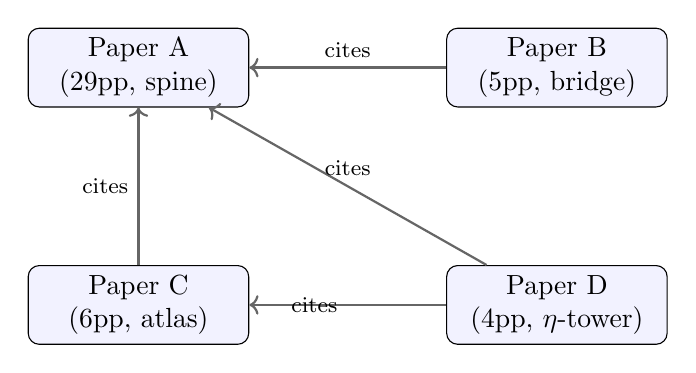
\begin{tikzpicture}[
  node distance=2.0cm and 2.5cm,
  paper/.style={draw, rectangle, rounded corners, minimum width=2.8cm, minimum height=1.0cm, align=center, fill=blue!5},
  cite/.style={->, thick, draw=black!60},
]
\node[paper] (A) {Paper A \\ (29pp, spine)};
\node[paper, right=of A] (B) {Paper B \\ (5pp, bridge)};
\node[paper, below=of A] (C) {Paper C \\ (6pp, atlas)};
\node[paper, right=of C] (D) {Paper D \\ (4pp, $\eta$-tower)};

\draw[cite] (B) -- node[above, sloped] {\footnotesize cites} (A);
\draw[cite] (C) -- node[left] {\footnotesize cites} (A);
\draw[cite] (D) -- node[above] {\footnotesize cites} (A);
\draw[cite] (D) -- node[left] {\footnotesize cites} (C);
\end{tikzpicture}
\end{center}

Paper A is the trunk. Papers B, C, D are independent companions, each
citing Paper A as mathematical input; Paper D additionally cites Paper C
for the atlas data. There are no circular dependencies; each companion
can be read after Paper A without the others.

\section{Consolidated open questions}

The four papers collectively pose six open mathematical questions,
ordered by tractability:

\begin{enumerate}[label=\textbf{(\Roman*)}, leftmargin=*, itemsep=4pt]
\item \textbf{Conjecture 16.5.2 (full $\mathrm{Sym}^{a}$ extension; Paper A).} Extend
the master quadratic uniqueness Theorem 16.5.1 from leading-period
polynomials to polynomials with arbitrary coefficients in $\mathrm{Sym}^{a}H^{1}$
and $\mathrm{Sym}^{b}H^{1}$. \emph{Estimated:} 2--4 months, requires
explicit period-algebra map.

\item \textbf{Cubic-AGM analog for $G_{\rho}$ (Paper A \S 17 P2).} For
$K = \Q(\rho)$, find an expression of the equianharmonic constant
$G_{\rho}$ in terms of the Borwein--Borwein cubic AGM iteration. The
Q(i) case has $\GG = 1/\mathrm{AGM}(1, \sqrt 2)$; the $\Q(
ho)$ analog is
not yet written down. \emph{Estimated:} weeks to months.

\item \textbf{Conjecture D.3.3 (higher-weight value algebras; Paper D).}
For each of the seven $w_K = 2$ class-number-one IQ fields, determine
the value algebra of $\{E_{2k}(\tau_K)\}_{k \geq 2}$ explicitly. The
natural framework is the level-$N$ modular value algebra at the
Atkin--Lehner fixed point. \emph{Estimated:} months per field.

\item \textbf{Conjecture 17.x ($W^{(4)}_{\mathrm{BCC}}$ algebraic
independence; Paper A).} $W^{(4)}_{\mathrm{BCC}} = (2/\pi)^{2}\,{}_4F_3(1/2^4; 1^3; 1)$
is algebraically independent of $\{\Gs, \pi, \Gamma(1/4)\}$. PSLQ at
$40$ digits gives no relation. \emph{Estimated:} requires modern
transcendence theory; multi-year.

\item \textbf{Conjecture 17.y (Catalan's constant; Paper A).}
$G_{\mathrm{Catalan}}$ is algebraically independent of $\{\GG, \pi\}$.
PSLQ at $80$ digits gives no relation. \emph{Estimated:} unknown;
even irrationality of $G_{\mathrm{Catalan}}$ is open.

\item \textbf{Open question E2 (CM Mahler measure; Paper D).} Develop a
tabulation of Laurent polynomials whose Mahler measures equal
Chowla--Selberg constants $\GK$, analogous to Boyd--Rodriguez-Villegas
for non-CM elliptic curves. \emph{Estimated:} unknown; new framework
required.

\item \textbf{Strict Kontsevich--Zagier period status of $\Gs$ (Paper A \S 17 P1).}
$\Gs \in \mathcal{P}^{\exp}$ unconditionally. Whether $\Gs \in \mathcal{P}$
(strict KZ-period) is conditional on $\sqrt{2\pi} \in \mathcal{P}$,
which is part of the broader KZ programme. \emph{Estimated:} not
tractable independently.
\end{enumerate}

Item (I) is the natural next target; closing it converts Paper A's central
theorem from leading-period restriction to full generality and unlocks
the Duke/JAMS-grade upgrade.

\section{Submission strategy}

\begin{center}
\renewcommand{\arraystretch}{1.3}
\begin{tabular}{>{\bfseries}l l l l}
\toprule
Paper & Primary target & Secondary & Notes \\
\midrule
A & Crelle (J.\ reine angew.\ Math.) & Compositio & Submit after final round of
copy-editing; Math.\ Ann.\ if Crelle declines on length grounds. \\
B & Foundations of Physics & J.\ Math.\ Phys.\ & Self-contained 5pp companion; format may require
journal-specific adjustments. \\
C & J.\ Number Theory & Acta Arithmetica & 6pp standalone; the $\GK$-table and Heegner Theorem 2.5 are
the contributions. \\
D & J.\ Number Theory & Math.\ Comp.\ & 4pp standalone; the $\eta$-tower formula
$|\eta(\tau_K)|^{2 w_K} = \GK^{w_K}/(2\pi|d_K|)^{w_K/2}$ is the contribution. \\
\bottomrule
\end{tabular}
\end{center}

\paragraph{Submission order.} Submit A first (it is cited by B, C, D as
the mathematical input). Submit B, C, D in parallel after Paper A's
status is known; each is self-contained relative to the published Paper A.
B, C, D can also be posted as a single arXiv preprint together with A
for cross-reference convenience before journal decisions arrive.

\paragraph{Duke / JAMS path.} The current Paper A is
\emph{Crelle / Compositio-grade}. Reaching Duke / JAMS requires closing
Conjecture 16.5.2 (the residual general-$\mathrm{Sym}^{a}$ case from
Theorem 16.5.1) or producing a comparable single deep new theorem at the
spine. This is a multi-month research push outside the present
opus's scope.

\section{Method note}

The opus was developed in a single intensive arc of authoring + multiple
rounds of specialist critique. Three lessons:

\paragraph{Specialist review catches what generalist review misses.} An
ivy-league CM-theorist critic identified a factor-of-2 error in
$L(E_{\mathrm{lemn}}, 1)$ that survived three prior rounds of generalist
polymath review. The fix changed $\varpi/2 \to \varpi/4$ in Paper A
\S 11, \S 16, and the compendium. (Independent mpmath verification:
LMFDB curve 32.a3 confirms $L(E, 1) = 0.6555\ldots = \varpi/4$.)

\paragraph{Explicit epistemic tagging prevents silent overclaim.} Every
substantive claim in the four papers carries one of:
$[\textsc{THEOREM}]$, $[\textsc{CONJECTURE}]$, $[\textsc{OBSERVATION}]$,
$[\textsc{SYNTHESIS}]$, $[\textsc{CLOSED NEGATIVE}]$. The Sym$^{2}\oplus$Sym$^{3}$
conjecture (Paper A \S 16.5) was initially stated as a conjecture; it
was refined into Theorem 16.5.1 (leading-period restriction) +
Conjecture 16.5.2 (general residual) once the proof scope was
isolated.

\paragraph{Negative results are documented.} The CM-internal candidates
for deriving the $(2, 3)$ exponent pair (Hilbert class polynomial,
$\eta$-quotient, Hecke eigenvalue, Petersson norm, Sym$^{2}$ L-value,
rank-twist, local invariants) were tested and found negative; the
explicit candidate list is preserved in Paper A \S 16.5 Remark
``three negative tests'' and the supporting scripts
\texttt{master\_quadratic\_from\_chi4.py} and
\texttt{master\_quadratic\_exponents\_2\_3.py}.

\section*{The four-paper bundle}

\begin{itemize}[leftmargin=*, itemsep=2pt]
\item \texttt{docs/papers/PAPER\_GSTAR\_INTRODUCTION.tex} (Paper A, 29pp)
\item \texttt{docs/papers/PAPER\_GSTAR\_FTD\_BRIDGE.tex} (Paper B, 5pp)
\item \texttt{docs/papers/PAPER\_GSTAR\_H1\_ATLAS.tex} (Paper C, 6pp)
\item \texttt{docs/papers/PAPER\_GSTAR\_ETA\_TOWER.tex} (Paper D, 4pp)
\item \texttt{docs/papers/PAPER\_GSTAR\_OPUS\_OVERVIEW.tex} (this document, the helper)
\end{itemize}

\end{document}
